\documentclass[]{article}
\usepackage{lmodern}
\usepackage{amssymb,amsmath}
\usepackage{ifxetex,ifluatex}
\usepackage{fixltx2e} % provides \textsubscript
\ifnum 0\ifxetex 1\fi\ifluatex 1\fi=0 % if pdftex
  \usepackage[T1]{fontenc}
  \usepackage[utf8]{inputenc}
\else % if luatex or xelatex
  \ifxetex
    \usepackage{mathspec}
  \else
    \usepackage{fontspec}
  \fi
  \defaultfontfeatures{Ligatures=TeX,Scale=MatchLowercase}
\fi
% use upquote if available, for straight quotes in verbatim environments
\IfFileExists{upquote.sty}{\usepackage{upquote}}{}
% use microtype if available
\IfFileExists{microtype.sty}{%
\usepackage{microtype}
\UseMicrotypeSet[protrusion]{basicmath} % disable protrusion for tt fonts
}{}
\usepackage[margin=1in]{geometry}
\usepackage{hyperref}
\hypersetup{unicode=true,
            pdftitle={Coursework 2},
            pdfauthor={Jennifer J. Stiens},
            pdfborder={0 0 0},
            breaklinks=true}
\urlstyle{same}  % don't use monospace font for urls
\usepackage{color}
\usepackage{fancyvrb}
\newcommand{\VerbBar}{|}
\newcommand{\VERB}{\Verb[commandchars=\\\{\}]}
\DefineVerbatimEnvironment{Highlighting}{Verbatim}{commandchars=\\\{\}}
% Add ',fontsize=\small' for more characters per line
\usepackage{framed}
\definecolor{shadecolor}{RGB}{248,248,248}
\newenvironment{Shaded}{\begin{snugshade}}{\end{snugshade}}
\newcommand{\KeywordTok}[1]{\textcolor[rgb]{0.13,0.29,0.53}{\textbf{#1}}}
\newcommand{\DataTypeTok}[1]{\textcolor[rgb]{0.13,0.29,0.53}{#1}}
\newcommand{\DecValTok}[1]{\textcolor[rgb]{0.00,0.00,0.81}{#1}}
\newcommand{\BaseNTok}[1]{\textcolor[rgb]{0.00,0.00,0.81}{#1}}
\newcommand{\FloatTok}[1]{\textcolor[rgb]{0.00,0.00,0.81}{#1}}
\newcommand{\ConstantTok}[1]{\textcolor[rgb]{0.00,0.00,0.00}{#1}}
\newcommand{\CharTok}[1]{\textcolor[rgb]{0.31,0.60,0.02}{#1}}
\newcommand{\SpecialCharTok}[1]{\textcolor[rgb]{0.00,0.00,0.00}{#1}}
\newcommand{\StringTok}[1]{\textcolor[rgb]{0.31,0.60,0.02}{#1}}
\newcommand{\VerbatimStringTok}[1]{\textcolor[rgb]{0.31,0.60,0.02}{#1}}
\newcommand{\SpecialStringTok}[1]{\textcolor[rgb]{0.31,0.60,0.02}{#1}}
\newcommand{\ImportTok}[1]{#1}
\newcommand{\CommentTok}[1]{\textcolor[rgb]{0.56,0.35,0.01}{\textit{#1}}}
\newcommand{\DocumentationTok}[1]{\textcolor[rgb]{0.56,0.35,0.01}{\textbf{\textit{#1}}}}
\newcommand{\AnnotationTok}[1]{\textcolor[rgb]{0.56,0.35,0.01}{\textbf{\textit{#1}}}}
\newcommand{\CommentVarTok}[1]{\textcolor[rgb]{0.56,0.35,0.01}{\textbf{\textit{#1}}}}
\newcommand{\OtherTok}[1]{\textcolor[rgb]{0.56,0.35,0.01}{#1}}
\newcommand{\FunctionTok}[1]{\textcolor[rgb]{0.00,0.00,0.00}{#1}}
\newcommand{\VariableTok}[1]{\textcolor[rgb]{0.00,0.00,0.00}{#1}}
\newcommand{\ControlFlowTok}[1]{\textcolor[rgb]{0.13,0.29,0.53}{\textbf{#1}}}
\newcommand{\OperatorTok}[1]{\textcolor[rgb]{0.81,0.36,0.00}{\textbf{#1}}}
\newcommand{\BuiltInTok}[1]{#1}
\newcommand{\ExtensionTok}[1]{#1}
\newcommand{\PreprocessorTok}[1]{\textcolor[rgb]{0.56,0.35,0.01}{\textit{#1}}}
\newcommand{\AttributeTok}[1]{\textcolor[rgb]{0.77,0.63,0.00}{#1}}
\newcommand{\RegionMarkerTok}[1]{#1}
\newcommand{\InformationTok}[1]{\textcolor[rgb]{0.56,0.35,0.01}{\textbf{\textit{#1}}}}
\newcommand{\WarningTok}[1]{\textcolor[rgb]{0.56,0.35,0.01}{\textbf{\textit{#1}}}}
\newcommand{\AlertTok}[1]{\textcolor[rgb]{0.94,0.16,0.16}{#1}}
\newcommand{\ErrorTok}[1]{\textcolor[rgb]{0.64,0.00,0.00}{\textbf{#1}}}
\newcommand{\NormalTok}[1]{#1}
\usepackage{graphicx,grffile}
\makeatletter
\def\maxwidth{\ifdim\Gin@nat@width>\linewidth\linewidth\else\Gin@nat@width\fi}
\def\maxheight{\ifdim\Gin@nat@height>\textheight\textheight\else\Gin@nat@height\fi}
\makeatother
% Scale images if necessary, so that they will not overflow the page
% margins by default, and it is still possible to overwrite the defaults
% using explicit options in \includegraphics[width, height, ...]{}
\setkeys{Gin}{width=\maxwidth,height=\maxheight,keepaspectratio}
\IfFileExists{parskip.sty}{%
\usepackage{parskip}
}{% else
\setlength{\parindent}{0pt}
\setlength{\parskip}{6pt plus 2pt minus 1pt}
}
\setlength{\emergencystretch}{3em}  % prevent overfull lines
\providecommand{\tightlist}{%
  \setlength{\itemsep}{0pt}\setlength{\parskip}{0pt}}
\setcounter{secnumdepth}{0}
% Redefines (sub)paragraphs to behave more like sections
\ifx\paragraph\undefined\else
\let\oldparagraph\paragraph
\renewcommand{\paragraph}[1]{\oldparagraph{#1}\mbox{}}
\fi
\ifx\subparagraph\undefined\else
\let\oldsubparagraph\subparagraph
\renewcommand{\subparagraph}[1]{\oldsubparagraph{#1}\mbox{}}
\fi

%%% Use protect on footnotes to avoid problems with footnotes in titles
\let\rmarkdownfootnote\footnote%
\def\footnote{\protect\rmarkdownfootnote}

%%% Change title format to be more compact
\usepackage{titling}

% Create subtitle command for use in maketitle
\newcommand{\subtitle}[1]{
  \posttitle{
    \begin{center}\large#1\end{center}
    }
}

\setlength{\droptitle}{-2em}

  \title{Coursework 2}
    \pretitle{\vspace{\droptitle}\centering\huge}
  \posttitle{\par}
    \author{Jennifer J. Stiens}
    \preauthor{\centering\large\emph}
  \postauthor{\par}
    \date{}
    \predate{}\postdate{}
  

\begin{document}
\maketitle

\subsection{Jennifer Stiens}\label{jennifer-stiens}

\href{mailto:j.j.stiens@gmail.com}{\nolinkurl{j.j.stiens@gmail.com}}

\href{https://github.com/jenjane118/ngs_tutorials}{github.com/jenjane118/ngs\_tutorials/coursework\_1.md}

\subsection{Question 1}\label{question-1}

\(\color{red}{\text{Compile a set of virulence-related genes in the AFPN02.1 strain and other E. coli strains and compare them}}\)

First I went to the VFPB website
(\url{http://www.mgc.ac.cn/VFs/main.htm}) and looked up `virulence
factors' associated with E. coli strains. The most common of these are:
adherence, toxin, invasion, Type III translocated protein, and immune
evasion. I can use these terms to annotate genes associated with
virulence.

\href{http://www.mgc.ac.cn/cgi-bin/VFs/genus.cgi?Genus=Escherichia}{VFDB
website, Escherichia Coli}

\(\color{red}{\text{a) Assemble a set of virulence-associated genes from public source or publication}}\)

From VFDB I was able to download a database of DNA sequences of core set
of experimentally-verified virulence-associated genes. This will be used
to extract genes (and relevant sequences) for the associated adhesion
genes for searching and annotating the AFPN02.1 genome.
(VFDB\_setA\_nt.fas) (\url{http://www.mgc.ac.cn/VFs/download.htm}) (Jin,
\emph{et.al.}, 2007).

Using the information on the VFDB website
(\url{http://www.mgc.ac.cn/cgi-bin/VFs/genus.cgi?Genus=Escherichia}),
Brzuszkiewicz, \emph{et. al.} (2011), and the spreadsheet of virulence
genes from EHEC and EAEC strains from Cheung, \emph{et.al}, (2011), I
compiled a list of 18 pertinent virulence-related genes. There were many
more genes available in the database, but these genes were selected
because they are related to adhesion and toxin production. I used the
gene names to select virulence-related genes from the VFDB.

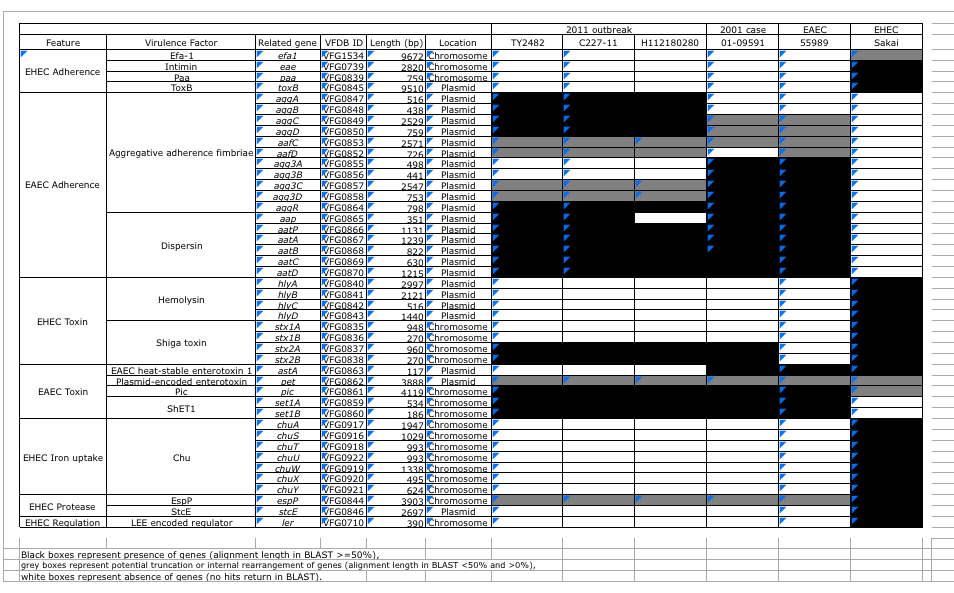
\includegraphics[width=0.75000\textwidth]{spreadsheet.png}
\(\begin{center} Virulence genes (Brzuszkiewicz, et al, 2011) \end{center}\)

\begin{Shaded}
\begin{Highlighting}[]
\CommentTok{## help for this code came from (https://infoplatter.wordpress.com/2013/10/15/extracting-specific-fasta-records-from-a-multi-fasta-file/)}
\CommentTok{## grabs all ecoli files and sequences}
\FunctionTok{awk} \StringTok{'BEGIN \{RS=">"\}/Escherichia/\{print">"$0\}'}\NormalTok{ VFDB_setA_nt.fas }\OperatorTok{>}\NormalTok{ ecoli_vfdb_genes.fas}
\CommentTok{## grabs all files with these genes}
\FunctionTok{cat}\NormalTok{ ecoli_vfdb_genes.fas }\KeywordTok{|} \FunctionTok{awk} \StringTok{'BEGIN \{RS=">"\}/aggR|agg3B|aat|astA|hlyA|sepA|aggA|setA|espP|setC|aat|fimH|fimA|cpxA|cpxR|csgA|elfA|stx/\{print">"$0\}'} \OperatorTok{>}\NormalTok{ virulence_vfdb_genes.fa}
\end{Highlighting}
\end{Shaded}

These have really elaborate headings, so I needed to make them much more
simple:

\begin{Shaded}
\begin{Highlighting}[]
\CommentTok{## removes part of heading before gene name}
\FunctionTok{cat}\NormalTok{ virulence_vfdb_genes.fa }\KeywordTok{|} \FunctionTok{sed} \StringTok{'s/^>.*(.*)\textbackslash{}s(//g'} \OperatorTok{>}\NormalTok{ temp.fa}
\CommentTok{## removes rest of heading after gene name}
\FunctionTok{cat}\NormalTok{ temp.fa }\KeywordTok{|} \FunctionTok{sed} \StringTok{'s/)\textbackslash{}s.*$//g'} \OperatorTok{>}\NormalTok{ virulence_vfdb_editedgenes.fa}
\FunctionTok{mv}\NormalTok{ virulence_vfdb_editedgenes.fa vfdb_virulence_genes.fa}
\end{Highlighting}
\end{Shaded}

\(\color{red}{\text{b) Build a separate set of virulence-associated genes in the annotation file created for AFPN02.1}}\)

The next step is to work with the annotation.gff file to retrieve
annotations based on `virulence', `adherence', `toxin', and `Type III'
(short for Type III aggregative adherence fimbriae) and convert into
.bed format.

\begin{Shaded}
\begin{Highlighting}[]
\FunctionTok{cat}\NormalTok{ annotation.gff }\KeywordTok{|} \FunctionTok{grep}\NormalTok{ -E }\StringTok{'virulence|adherence|toxin|invasion|Type III'} \KeywordTok{|} \FunctionTok{awk} \StringTok{'BEGIN \{FS="\textbackslash{}t"\}  split($9, captured, /[(=);]/) >=10  \{print "sequence1" "\textbackslash{}t" $4 "\textbackslash{}t" $5 "\textbackslash{}t" captured[10] "\textbackslash{}t" captured[4] "\textbackslash{}t" $7\}'} \OperatorTok{>}\NormalTok{ present_in_AFPN02_virulence_genes.bed}
\end{Highlighting}
\end{Shaded}

Then we have to retrieve the DNA sequence for these genes and save in
fasta format:

\begin{Shaded}
\begin{Highlighting}[]
\ExtensionTok{/s/software/bedtools/v2.27.1/bin/bedtools}\NormalTok{ getfasta -name -s -fi }\VariableTok{$\{st_path\}}\NormalTok{/results_GC/annotation/genome.fna -bed present_in_AFPN02_virulence_genes.bed -fo present_in_AFPN02_virulence_genes.fasta}
\end{Highlighting}
\end{Shaded}

A bit more formatting to get rid of extra elements in the heading:

\begin{Shaded}
\begin{Highlighting}[]
\FunctionTok{cat}\NormalTok{ present_in_AFPN02_virulence_genes.fasta }\KeywordTok{|} \FunctionTok{sed} \StringTok{'s/(.*//g'} \OperatorTok{>}\NormalTok{ present_in_AFRN02_virulence_genes.fasta}
\end{Highlighting}
\end{Shaded}

Then we have to combine the two files:

\begin{Shaded}
\begin{Highlighting}[]
\FunctionTok{cat}\NormalTok{ present_in_AFPN02_virulence_genes.fasta vfdb_virulence_genes.fa }\OperatorTok{>}\NormalTok{ final_comparison_virulence.fasta}
\FunctionTok{cp}\NormalTok{ present_in_AFPN02_virulence_genes.fasta vfdb_virulence_genes.fa final_comparison_virulence.fasta }\VariableTok{$\{st_path\}}\NormalTok{/results_GC/wholeGenomeExamples}
\end{Highlighting}
\end{Shaded}

\(\color{red}{\text{c) Use BRIG to visualise which of the virulence genes are present/absent in E. coli strains}}\)

To run brig, use the following command:

\begin{Shaded}
\begin{Highlighting}[]
\ExtensionTok{/s/software/brig/BRIG-0.95-dist/brig.sh}
\end{Highlighting}
\end{Shaded}

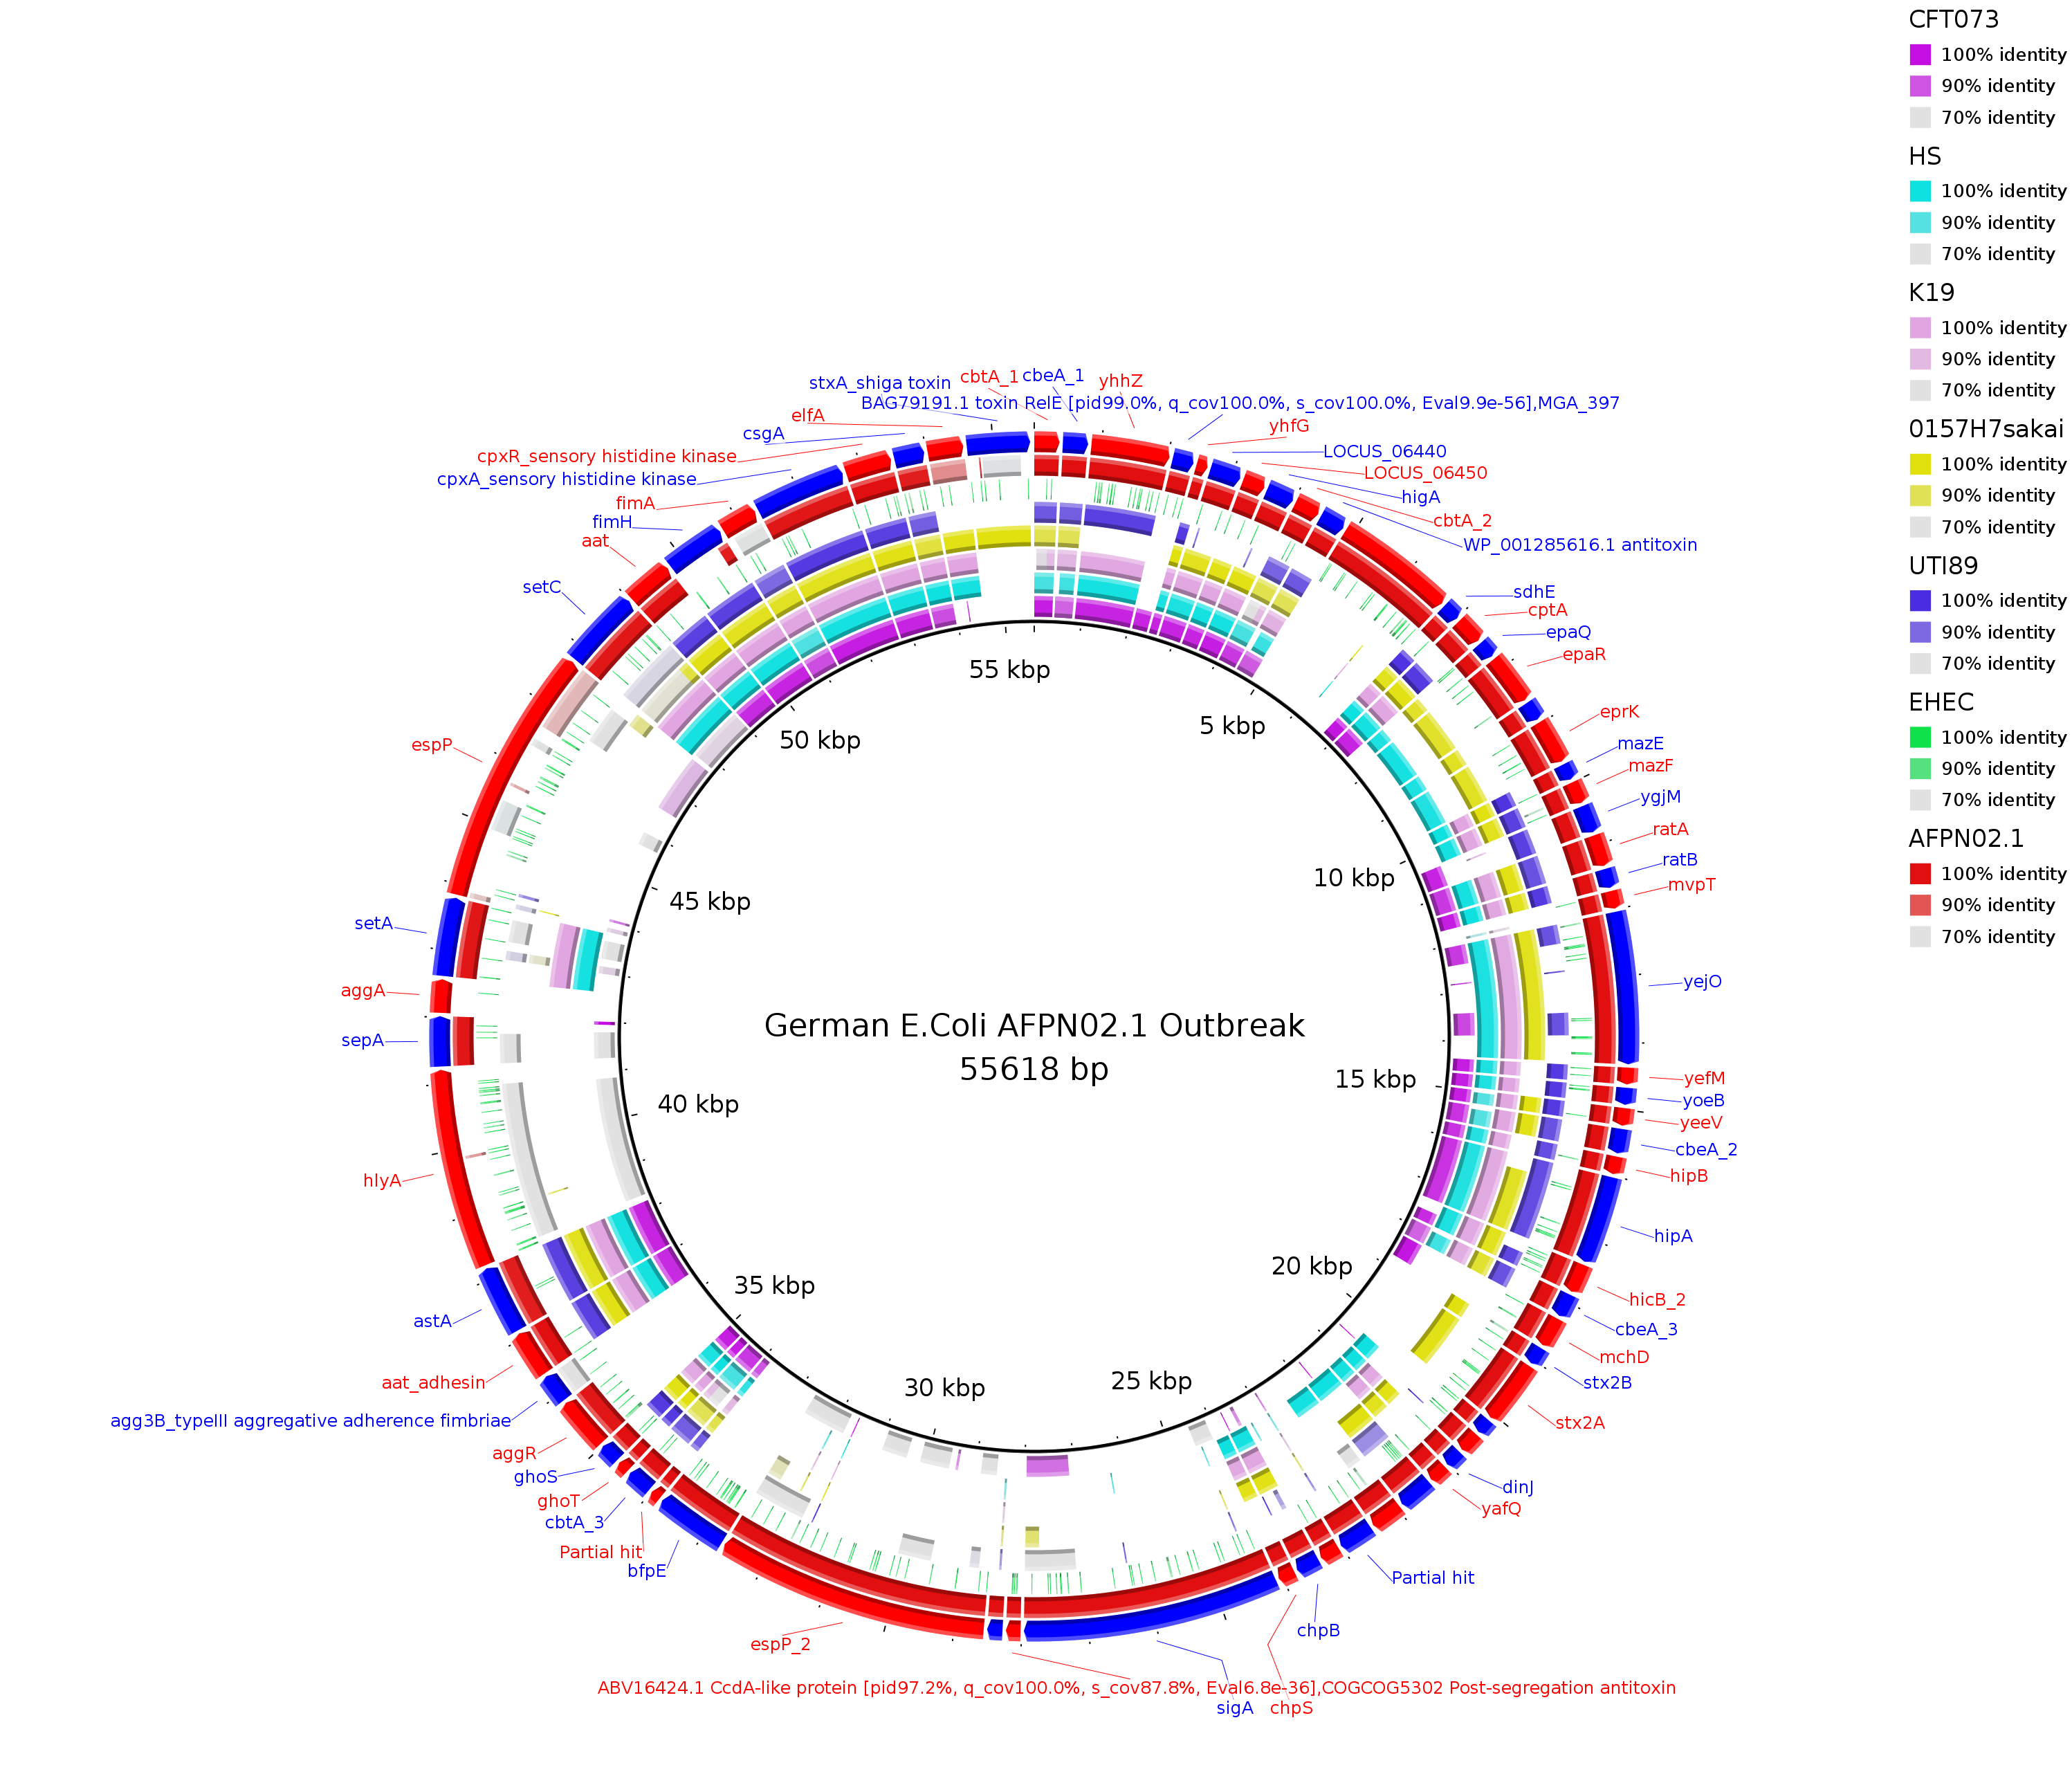
\includegraphics{final_comparison_virulence.fasta.png}

\begin{center} BRIG: Blast Ring Image Generator (brig.sourceforge.net) \end{center}

Most of the virulence genes were present in AFPN02.1. However, hylA was
only identified with a short sequence, aggA was completely missing, esp
was mostly missing, though some parts were present at lower identity,
fimH was completely missing, stxA was more weakly identified, and agg3B
was more weakly identified. The other shiga-toxin genes, stx2A/B were
present in the AFPN02.1 strain, as well as in the sakai strain, which is
a EHEC (enterohemmoragic) strain, but isn't present at all in the other
strains, except for short regions of identity with the other EHEC
strain. The EHEC strain seemed the most different from the other
strains, with only short regions of identity spread out over the genome,
however, it seemed there were hits in all of the genes.

\subsection{Question 2}\label{question-2}

\(\color{red}{\text{Select ONE of the virulence genes (or if you prefer one operon) present in AFPN02.1
and study this}}\)
\(\color{red}{\text{gene/operon in more detail including its biological action/mechanism phylogeny.}}\)

\subsection{References}\label{references}

Brzuszkiewicz, E., Thürmer, A., Schuldes, J., Leimbach, A., Liesegang,
H., Meyer, F.-D., \ldots{} Daniel, R. (2011). Genome sequence analyses
of two isolates from the recent Escherichia coli outbreak in Germany
reveal the emergence of a new pathotype: Entero-Aggregative-Haemorrhagic
Escherichia coli (EAHEC). Archives of Microbiology, 193(12), 883--891.
\url{https://doi.org/10.1007/s00203-011-0725-6}

Cheung, M., Li, L., Nong, W., \& Kwan, H. (2011). 2011 German
Escherichia coli O104:H4 outbreak: Whole-genome phylogeny without
alignment. BMC Research Notes, 4(December).
\url{https://doi.org/10.1186/1756-0500-4-533}

`Enteroaggregative Escherichia coli.' Wikipedia: The Free Encyclopedia.
Wikipedia, The Free Encyclopedia, 28 January 2019,
en.wikipedia.org/wiki/Enteroaggregative\_Escherichia\_coli

Jin, Q., Sun, L., Yang, J., Chen, L., \& Yu, J. (2007). VFDB 2008
release: an enhanced web-based resource for comparative pathogenomics.
Nucleic Acids Research, 36(Database), D539--D542.
\url{https://doi.org/10.1093/nar/gkm951}


\end{document}
